\documentclass[11pt]{amsart}
\usepackage{amsfonts,amsbsy}
\usepackage[pdftex]{graphicx}
\usepackage{amsaddr}
\usepackage{setspace}
\usepackage{caption}
%\usepackage[margin=1.5in]{geometry}

\usepackage[framemethod=tikz,innerleftmargin=0]{mdframed}




\newcommand{\N}{\mathcal{N}}
\newcommand{\want}{p^{\epsilon}}
\newcommand{\noise}{\sqrt{\epsilon}}
\newcommand{\E}{\mathbb{E}}
\newcommand{\ind}{\mathbf{1}}
\newcommand{\R}{\mathbb{R}}


\newcommand{\kknote}[1]{{\textcolor{magenta}{#1}}}
\newcommand{\ydnote}[1]{{\textcolor{cyan}{#1}}}
\newcommand{\dmnote}[1]{{\textcolor{green}{#1}}}

% bibliography
% \usepackage[style=authoryear,backend=bibtex,natbib=true]{biblatex}

% \renewbibmacro{in:}{}

% \addbibresource{refs.bib}

% theorem commands 


\begin{document}

\title{Exercise}

\author{Yair Daon, Karina Koval}
\address{Courant Institute of Mathematical Sciences \\ New York University \\ 251 Mercer St., New York, NY}


\thanks{Me!!!} 
\date{\today}

\begin{abstract}
  A write up of the exercise for Eric's class.
\end{abstract}


\maketitle


\section{Hi}
\ydnote{This is my note}. \kknote{This is KKK's note}. \dmnote{Guess what this is}.
%\onehalfspacing
\section{Problem}
Suppose you have a particle moving according to the following SDE:

\begin{align*}
  dX_t = \noise dW_t,
\end{align*}
with $W_t$ Brownian motion. The process starts at $x \in (0,1)$. We are
interested in 

\begin{align*}
  \want = \Pr( |X_1| > 1 ) =:\Pr(A). 
\end{align*}
Note that
\begin{equation}
\want = 2 \int_{1}^{\infty} e^{-\frac{1}{2\epsilon}(y-x)^2} \frac{dy}{\sqrt{2\pi\epsilon}} 
\end{equation}

\section{Naiive estimator}
The naive estimator will require an exponential number of samples since 
$X_1 \sim \N( x, \epsilon )$ and $A$ is a rare event.

\section{Second Estimator}
We can use the instanton 
\begin{align*}
  \phi(t) = (1-t)x + t
\end{align*}
and generate the biased process
\begin{align*}
dY_t = \dot{\phi}(t)dt + \noise dW_t
\end{align*}
which also starts at $x$. The process is
\begin{align*}
  Y_t = (1-t)x + t + \noise W_t
\end{align*}
and
\begin{align*}
  Y_1 = 1 + \noise W_1.
\end{align*}

\subsection{Girsanov}
Girsanov's theorem (Oksendal, Theorem 8.6.6) states (in 1D, without details)
the following. Let $Y_t$ an Ito process of the form
\begin{align*}
  dY_t = \beta(t,\omega)dt + \theta(t,\omega) dB_t
\end{align*} 
and 
\begin{align*}
  \theta(t,\omega) u(t,\omega) = \beta(t,\omega) - \alpha(t,\omega).
\end{align*}
Take
\begin{align*}
  M_t = \exp \bigg ( 
  - \int_0^t u(s,\omega) dB_s -\frac{1}{2} \int_0^t u^2(s,\omega) ds 
  \bigg )
\end{align*}
and $d\mathbb{Q}(\omega) = M_T d\mathbb{P}(\omega)$. Then 
\begin{align*}
  \hat{B}_t : = \int_0^t u(s,\omega) ds + B_t 
\end{align*}
is BM wrt $\mathbb{Q}$ and
\begin{align*}
  dY_t = \alpha(t,\omega) dt + \theta( t,\omega )d\hat{B}_t.
\end{align*}

\subsection{In our case}
In our case $dX_t = \noise dW_t$, so $\beta \equiv 0$ and $\theta \equiv \noise$.
We want to finish with a new process with $\alpha = \dot{\phi}$ so this can only
mean $u = -\frac{\dot{\phi}(t)}{\noise}$. Thus
\begin{align*}
  M_t &= \exp \bigg ( - \int_0^t -\frac{\dot{\phi}(t)}{\noise}dW_s 
  -\frac{1}{2} \int_0^t \frac{\dot{\phi}^2(t)}{\epsilon}ds \bigg ) \\
  %
  %
  %
  &=  \exp \bigg ( \frac{1}{\noise} \int_0^t \dot{\phi}(t)dW_s 
  -\frac{1}{2\epsilon} \int_0^t \dot{\phi}^2(t)ds \bigg ). \\
\end{align*}
%
We record the explicit expression we use:
%
\begin{align}\label{eq:explicit M}
  M_{T=1}^{-1} &= \exp \bigg ( \frac{x-1}{\noise} W_1 
  +\frac{(1-x)^2}{2\epsilon}  \bigg ).
\end{align}
%
We want to calculate the following:
%
\begin{align*}
  \want = \mathbb{P}(A) = \int_A d\mathbb{P}(\omega) = 
  \int_A M_{T=1}^{-1} d\mathbb{Q}(\omega) = \E_{\mathbb{Q}}[\ind_{A} M_{T=1}^{-1}].
\end{align*}
Under $\mathbb{Q}$, we know that $dX_t = \dot{\phi}(t) + \noise d\hat{W}_t$, so 
we can just call it $Y_t$ and drop the hat on $W$ (as we did above). If we do that,
then $dY_t = \dot{\phi}(t) + \noise dW_t$ and:
\ydnote{given expression \eqref{eq:explicit M} this is redundant I think...}
\begin{align}
  \begin{split}
  \want &= \E\left [ \ind_{ |Y_t| > 1 } \exp \left (
      -\frac{1}{\noise} \int_0^1 \dot{\phi}(s)dW_s  
      +\frac{1}{2\epsilon} \int_0^1 \dot{\phi}^2(s)ds \right ) \right ] \\
  %
  %
  %
  &= \E\left [ \ind_{ |Y_t| > 1 } \exp \left (
      -\frac{1}{\noise} \int_0^1 (1-x) dW_s  
      +\frac{1}{2\epsilon} \int_0^1 (1-x)^2 ds \right ) \right ] \\
  %
  %
  %
  &= \E\left [ \ind_{ |Y_t| > 1 } \exp \left (
      -\frac{1-x}{\noise} W_1 +\frac{(1-x)^2}{2\epsilon} \right ) \right ] \\
  %
  %
  %
  &= \E\left [ \ind_{ |Y_t| > 1 } \exp \left (
     \frac{x-1}{\noise} W_1 +\frac{(1-x)^2}{2\epsilon} \right ) \right ] \\
 \end{split}
\end{align}

\subsection{First Moment}
Let $ A = \{ Y : |Y| \geq 1 \}$. Noting that $Y_1 = 1 + \noise W_1$
we have that: 
\begin{align}
  \E\left [ \ind_{ |Y_t| > 1 } \exp \left (
     \frac{x-1}{\noise} W_1 +\frac{(1-x)^2}{2\epsilon} \right ) \right ] =
   \int_{\R} \ind_{A}(1+\noise z)\exp^{-(\frac{(1-x)z}{\noise}+\frac{(1-x)^2}{2\epsilon}+\frac{z^2}{2})} \frac{dz}{\sqrt{2\pi}} \\
\end{align}
Letting $z = \frac{y-1}{\noise} \implies dz = \frac{dy}{\noise} \implies $ 
\begin{align}
  \begin{split}
    \want &= \int_{\R} \ind_{A}(y)
    \exp^{-(\frac{(1-x)(y-1)}{\epsilon}+\frac{(1-x)^2}{2\epsilon}+\frac{(y-1)^2}{2\epsilon})}
    \frac{dy}{\sqrt{2\pi\epsilon}} \\
    %
    %
    %
    &= \int_{\R} \ind_{A}(y)
    \exp^{-\frac{1}{2\epsilon} (-2 - 2xy +2x +2y + 1 + x^2 -2x + 1 +y^2 -2y  )}
    \frac{dy}{\sqrt{2\pi\epsilon}} \\ 
    %
    %
    %
    &= \int_{\R} \ind_{A}(y) \exp^{-\frac{(y-x)^2}{2\epsilon}}
    \frac{dy}{\sqrt{2\pi\epsilon}} \\
    %
    %
    %
    &= 2\int_{1}^{\infty} \exp^{-\frac{(y-x)^2}{2\epsilon}}
    \frac{dy}{\sqrt{2\pi\epsilon}} \\
    %
    %
    %
    &= \Pr( |X_1| > 1 ) \\
  \end{split}
\end{align}
Thus $\E_{\mathbb{Q}}[\ind_{A}(Y_1) M_{T=1}^{-1}]$ is an unbiased estimator. 

\subsection{Second Moment}
Now we compute the second moment for
$\Theta :=\ind_{A}(Y_1) M_{T=1}^{-1}$.
\ydnote{you dont compute the second moment of a number, but that of
  a RV, hence I removed the expectation. Similarly below, I replaced
  $\want^2$}
\begin{align}
  \begin{split}
    \E_{\mathbb{Q}}[\Theta^2]
    &= \E_{\mathbb{Q}}[\ind_{A}^2(Y_1) M_{T=1}^{-2}] \\
    %
    %
    %
    &= \int_{\R} \ind_{A}(1+\noise z)
    \exp^{-\frac{2(1-x)z}{\noise}-\frac{(1-x)^2}{\epsilon}-\frac{z^2}{2}}
    \frac{dz}{\sqrt{2\pi}} \\
  \end{split}
\end{align}
Letting $y = \noise z \implies dz = \frac{dy}{\noise}$
\begin{align}
  \begin{split}
    \E_{\mathbb{Q}}[\Theta^2]
    &= \int_{\R} \ind_{A}(1+y)
    \exp^{-\frac{1}{2}(\frac{4(1-x)y}{\epsilon}+\frac{2(1-x)^2}{\epsilon}+\frac{y^2}{\epsilon})}
    \frac{dy}{\sqrt{2\pi\epsilon}} \\
    %
    %
    %
    &= \int_{\R} \ind_{A}(1+y)
    \exp^{\frac{-(y+2(1-x))^2}{2\epsilon}+\frac{(1-x)^2}{\epsilon}}
    \frac{dy}{\sqrt{2\pi\epsilon}}\\
    %
    %
    %
    &= (\int_{-\infty}^{-2}+\int_{0}^{\infty})
    \exp^{\frac{-(y+2(1-x))^2}{2\epsilon}+\frac{(1-x)^2}{\epsilon}}
    \frac{dy}{\sqrt{2\pi\epsilon}}\\
  \end{split}
\end{align}
Where the second equality comes from the fact that
$y^2+4(1-x)y+2(1-x)^2=(y+2(1-x))^2-2(1-x)^2$.

Letting $z = y+2(1-x) \implies$
\begin{align}
  \begin{split}
    \E_{\mathbb{Q}}[\Theta^2]
    &= (\int_{-\infty}^{-2x}+\int_{2-2x}^{\infty})
    \exp^{\frac{-z^2}{2\epsilon}+\frac{(1-x)^2}{\epsilon}}
    \frac{dz}{\sqrt{2\pi\epsilon}} \\
    %
    %
    %
    &= (\int_{2x}^{\infty}+\int_{2-2x}^{\infty})
    \exp^{\frac{-z^2}{2\epsilon}+\frac{(1-x)^2}{\epsilon}}
    \frac{dz}{\sqrt{2\pi\epsilon}} \\
  \end{split}
\end{align}
%
%
\begin{figure}[h]
\caption{Plot of $z = 2x$ and $z = 2-2x$}
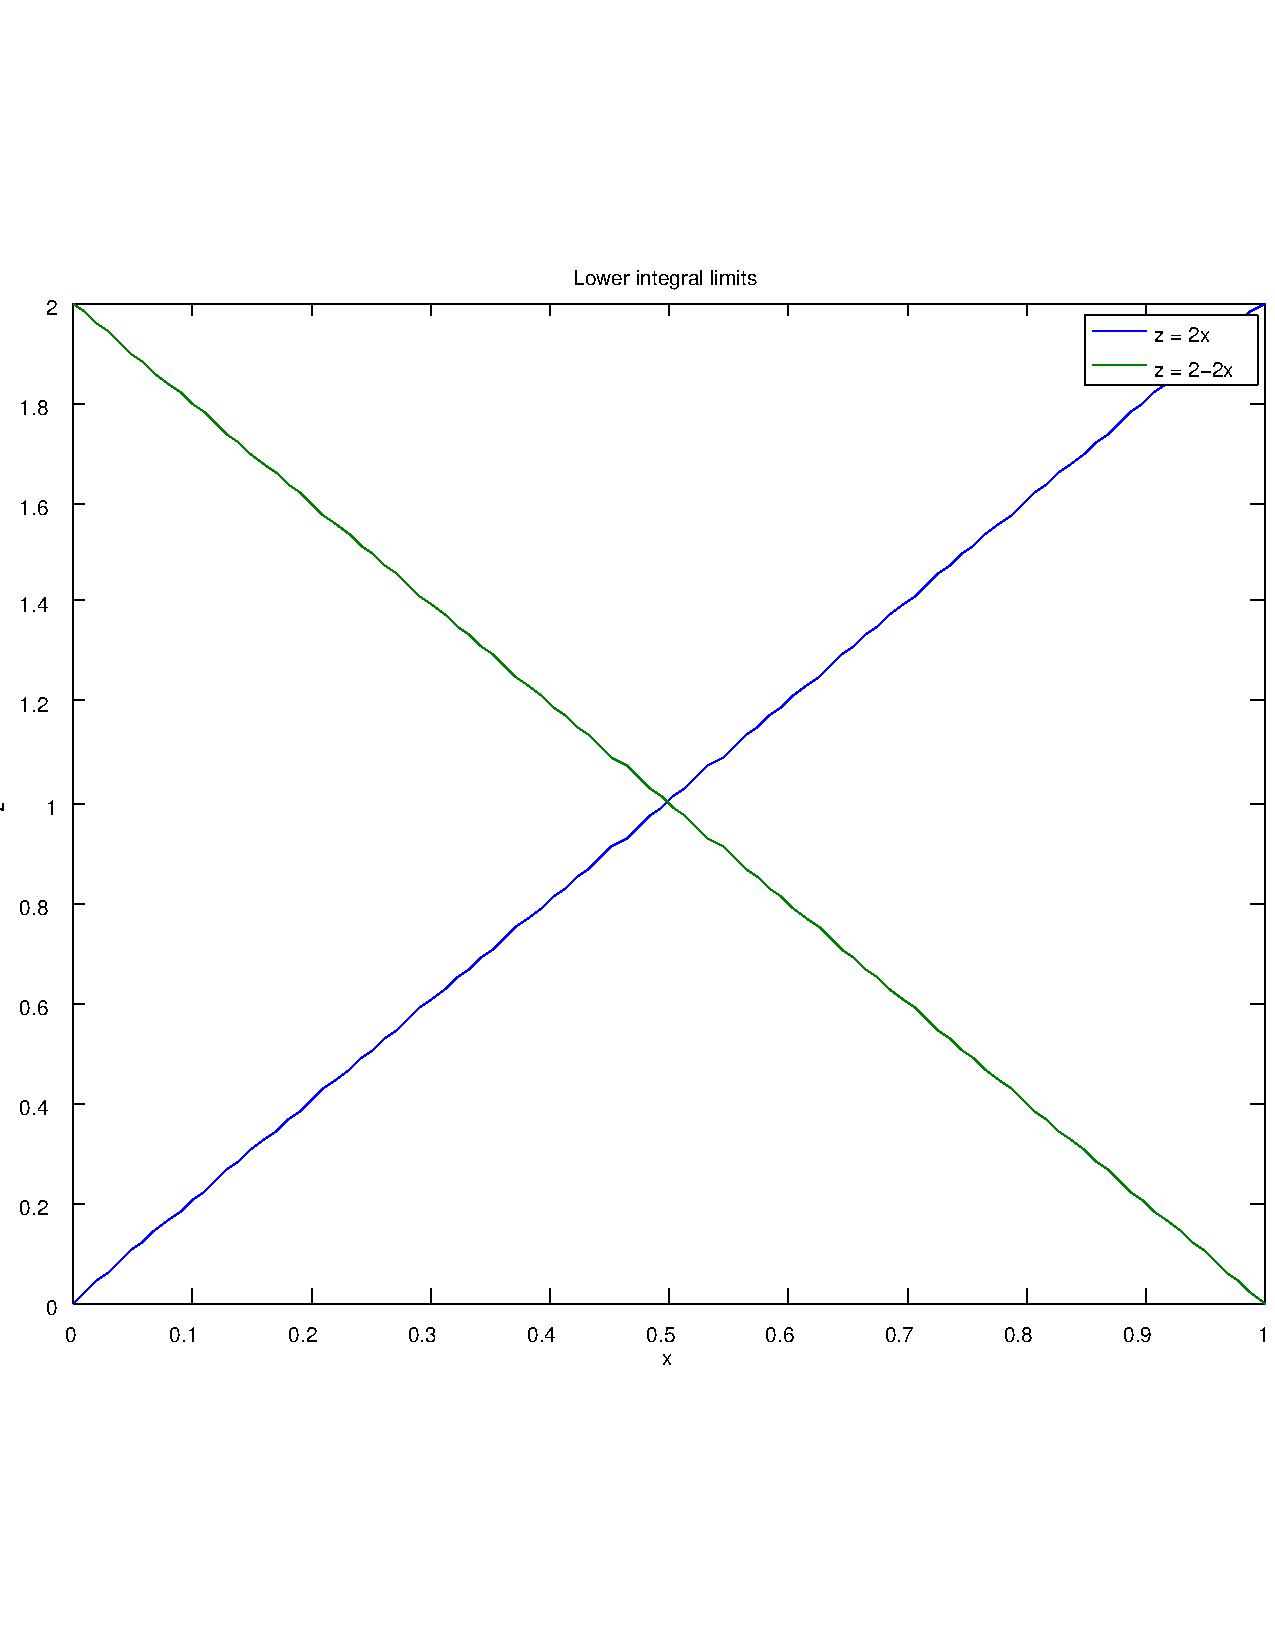
\includegraphics[scale=0.4]{plot.pdf}
\end{figure}
%
%
Looking at figure 1, we can see that for small enough
$\epsilon$, the second moment is dominated by different
values depending on $x$. There are two cases to consider: 
\\
For $1 > x > \frac{1}{2}$, $(\want)^2(x) \asymp \exp^{\frac{(1-x)^2}{\epsilon}-\frac{(2-2x)^2}{2\epsilon}} = \exp^{-\frac{(x-1)^2}{\epsilon}} \implies \lim_{\epsilon \to 0} (\want)^2 = 0$
\\
For $0 < x < \frac{1}{2}$, $(\want)^2(x) \asymp \exp^{\frac{(1-x)^2}{\epsilon}-\frac{(2x)^2}{2\epsilon}} = \exp{\frac{1-2x-x^2}{\epsilon}}$. For $x \in (0,\sqrt{2}-1]$, $1-2x-x^2 > 0 \implies \lim_{\epsilon \to 0} (\want)^2(x) = \infty$ 
\\
Thus, the relative error of the estimator, which is $\text{Rel. error} = \frac{(\want)^2}{N\int_{\R}\ind_{A}(Y)M^{-1}_{T}(Y) dY} \to \infty$ as $\epsilon \to 0$. This is not generally a good method to approximate $P(A)$ in practice. 

\section{Better Estimator}
Consider the process: 
\begin{align*}
dZ_t = (1-Z_t)dt + \noise dW_t
\end{align*}

\kknote{Anyone want to start this part up? i.e., use Girsanov to write out $M_T$ for this process?}
\ydnote{We can do it. Stronger, together.}
%\printbibliography

\end{document}

